% Title: glps_renderer figure
% Creator: GL2PS 1.3.8, (C) 1999-2012 C. Geuzaine
% For: Octave
% CreationDate: Thu Nov 13 09:45:59 2014
\setlength{\unitlength}{1pt}
\begin{picture}(0,0)
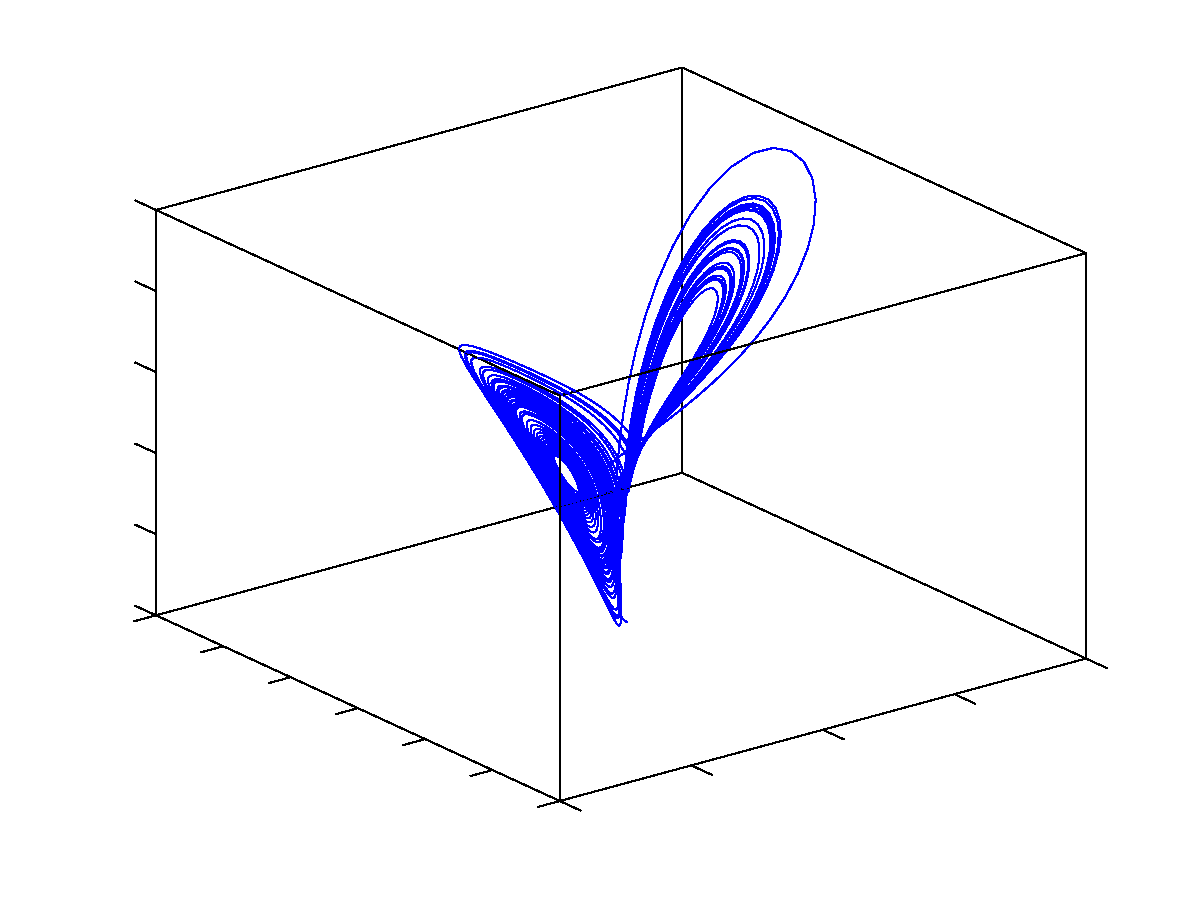
\includegraphics{CurvaLorentz-inc}
\end{picture}%
\begin{picture}(576,432)(0,0)
\fontsize{10}{0}
\selectfont\put(188.51,73.009){\makebox(0,0)[tr]{\textcolor[rgb]{0,0,0}{{-10}}}}
\fontsize{10}{0}
\selectfont\put(156.207,87.8628){\makebox(0,0)[tr]{\textcolor[rgb]{0,0,0}{{0}}}}
\fontsize{10}{0}
\selectfont\put(123.905,102.716){\makebox(0,0)[tr]{\textcolor[rgb]{0,0,0}{{10}}}}
\fontsize{10}{0}
\selectfont\put(91.602,117.57){\makebox(0,0)[tr]{\textcolor[rgb]{0,0,0}{{20}}}}
\fontsize{10}{0}
\selectfont\put(59.2995,132.424){\makebox(0,0)[tr]{\textcolor[rgb]{0,0,0}{{30}}}}
\fontsize{10}{0}
\selectfont\put(220.812,58.1553){\makebox(0,0)[tr]{\textcolor[rgb]{0,0,0}{{-20}}}}
\fontsize{10}{0}
\selectfont\put(60.2059,143.39){\makebox(0,0)[br]{\textcolor[rgb]{0,0,0}{{0}}}}
\fontsize{10}{0}
\selectfont\put(60.2059,182.304){\makebox(0,0)[br]{\textcolor[rgb]{0,0,0}{{10}}}}
\fontsize{10}{0}
\selectfont\put(60.2059,221.219){\makebox(0,0)[br]{\textcolor[rgb]{0,0,0}{{20}}}}
\fontsize{10}{0}
\selectfont\put(60.2059,260.133){\makebox(0,0)[br]{\textcolor[rgb]{0,0,0}{{30}}}}
\fontsize{10}{0}
\selectfont\put(60.2059,299.047){\makebox(0,0)[br]{\textcolor[rgb]{0,0,0}{{40}}}}
\fontsize{10}{0}
\selectfont\put(60.2059,337.962){\makebox(0,0)[br]{\textcolor[rgb]{0,0,0}{{50}}}}
\fontsize{10}{0}
\selectfont\put(298.08,409.6){\makebox(0,0)[b]{\textcolor[rgb]{0,0,0}{{Curva de Lorentz con parámetros $\alpha=10$, $\beta=28$ y $\rho=\frac{8}{3}$}}}}
\fontsize{10}{0}
\selectfont\put(253.115,43.3016){\makebox(0,0)[tr]{\textcolor[rgb]{0,0,0}{{-30}}}}
\fontsize{10}{0}
\selectfont\put(283.369,40.7724){\makebox(0,0)[tl]{\textcolor[rgb]{0,0,0}{{-20}}}}
\fontsize{10}{0}
\selectfont\put(346.515,57.8688){\makebox(0,0)[tl]{\textcolor[rgb]{0,0,0}{{-10}}}}
\fontsize{10}{0}
\selectfont\put(409.662,74.9653){\makebox(0,0)[tl]{\textcolor[rgb]{0,0,0}{{0}}}}
\fontsize{10}{0}
\selectfont\put(472.808,92.0618){\makebox(0,0)[tl]{\textcolor[rgb]{0,0,0}{{10}}}}
\fontsize{10}{0}
\selectfont\put(535.954,109.158){\makebox(0,0)[tl]{\textcolor[rgb]{0,0,0}{{20}}}}
\end{picture}
